\documentclass{beamer}
\usepackage[utf8]{inputenc}
\usepackage{graphicx}
\usepackage{listings}
\usetheme[]{boxes}
\usecolortheme{seagull}
%\usepackage{french}
\title{Programmation OpenMP}
\author{Marc Tajchman}\institute{CEA - DEN/DM2S/STMF/LMES}
\date{30 novembre 2018}
\begin{document}

\begin{frame}
\titlepage
\end{frame}

\Large
\begin{frame}
  	\tableofcontents
\end{frame}

\begin{frame}
\section{Rappels sur OpenMP - Exemples commentés}
\frametitle{Rappels sur l'architecture mat\'erielle}
\textcolor{blue}{On peut voir la structure d'une machine de calcul \`a diff\'erentes \'echelles}:
\vfill

Vue globale: un ensemble de n\oe uds de calcul chacun contenant un ou plusieurs processeurs et de la m\'emoire, les n\oe uds sont connect\'es par un r\'eseau:

\vfill
\begin{center}
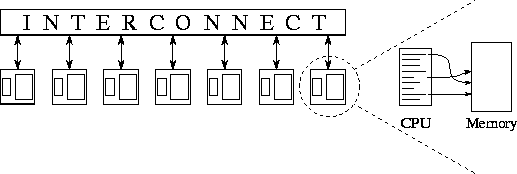
\includegraphics[scale=0.4]{../Images/img100}
\end{center}

(les machines les plus puissantes actuellement contiennent plusieurs centaines de milliers de n\oe uds)
\end{frame}

\begin{frame}
Vue interne d'un n\oe ud (variable suivant le mod\`ele de processeur et la g\'en\'eration utilis\'ee):

\begin{center}
\includegraphics[scale=0.3]{../Images/architecture2}
\end{center}

\end{frame}

\begin{frame}
Vue interne d'un c\oe ur (variable suivant le mod\`ele de processeur et la g\'en\'eration utilis\'ee):

\begin{center}
	\includegraphics[scale=0.18]{../Images/1106px-zen_block_diagram}
	
	AMD - Zen $\mu$arch
\end{center}

\end{frame}

\begin{frame}[fragile]
Situation actuelle (et encore pour plusieurs ann\'ees): 
\begin{quote}
	
	\vfill
	vitesse de calcul (d'un processeur)
	\vfill
	
	\begin{itemize}
		\item[$\approx$] vitesse de la m\'emoire interne (registres) du processeur
			\medskip
	        
		\item[$>$] vitesse des diff\'erentes m\'emoires cache, interm\'ediaires entre le processeur et la m\'emoire centrale du n\oe ud (
		
		\hfill vitesse L1 $>$ L2 $>$ L3, 
		
		\hfill taille L1 $<$ L2 $<$ L3)
			\medskip
			
		\item[$\gg$] vitesse de la m\'emoire centrale d'un n\oe ud
			\medskip
			
		\item[$\gg$] vitesse du r\'eseau qui connecte les n\oe uds
	\end{itemize}


\end{quote}

\end{frame}

\begin{frame}
Fonctionnement :

\begin{itemize}
	\item Quand un c\oe ur  a besoin d'une donn\'ee, il la demande au gestionnaire m\'emoire.
	\vfill
	
	\item Le gestionnaire m\'emoire regarde si la donn\'ee est dans la m\'emoire cache L1, L2 ou L3 de ce processeur, sinon le bloc de la m\'emoire centrale qui contient la donn\'ee est recopi\'e dans la m\'emoire cache (dans L3, puis L2 et  L1).
	
	\vfill
	\item Ensuite, la donn\'ee est recopi\'ee dans un registre de ce c\oe ur.
	
	\vfill
\end{itemize}
\end{frame}

\begin{frame}

\vfill
\begin{itemize}
\item Quand un c\oe ur a modifi\'e une donn\'ee, il le notifie au gestionnaire m\'emoire
\vfill
\item Le gestionnaire m\'emoire recopie la donn\'ee vers la m\'emoire cache (L1, L2 puis L3) et vers la m\'emoire centrale
\vfill
\item Il v\'erifie aussi qu'une autre copie de la donn\'ee n'existe pas dans la m\'emoire cache d'un autre c\oe ur.
\vfill
\item Si c'est la cas, les autres copies sont mises \`a jour
\end{itemize}
	\vfill
\end{frame}

\begin{frame}[fragile]
	
	\vfill
{\bf Cette gestion peut repr\'esenter une partie im\-por\-tante du temps d'ex\'ecution (pour assurer la coh\'erence des diff\'erentes parties de la m\'emoire et leurs mises \`a jour correctes).}
	\vfill


\end{frame}

\begin{frame}
\section{Programmation s\'equentielle efficace}
\frametitle{Programmation s\'equentielle efficace}

\bf
\textcolor{blue}{Pour obtenir un code efficace (en temps d'ex\'ecution), il faut:}

\begin{itemize}
	\item utiliser les algorithmes les plus efficaces possible (pas couvert par ce cours)
	
	\item organiser le placement des donn\'ees (am\'eliorer la localit\'e spatiale)
	
	\item organiser la s\'equence d'instructions (am\'eliorer la localit\'e temporelle)

	\item \'ecrire les instructions pour qu'elles soient les plus rapides (utilisation du // interne des processeurs, \'eviter si possible les tests)
\end{itemize}
\end{frame}

\begin{frame}
\frametitle{Localit\'e spatiale}
Règle:  \textcolor{red}{autant que possible, utiliser des zones m\'emoires proches les unes des autres dans une s\'equence d'instructions}
\begin{quote}
	Le transfert entre m\'emoire centrale et m\'emoire cache se fait par bloc de donn\'ees.
	
	Donc, si une donn\'ee est \`a c\^ot\'e d'une donn\'ee qui vient d'\^etre utilis\'ee (et donc transf\'er\'ee en m\'emoire cache), un nouveau transfert sera peut-\^etre inutile.
\end{quote}

\vfill
Exemple: voir TP 1
\end{frame}

\begin{frame}
\frametitle{Localit\'e temporelle}
Règle: 
	\textcolor{red}{autant que possible, pour une zone m\'emoire, les instructions qui l'utilisent doivent s'ex\'ecuter de façon rapproch\'ee dans le temps}
	
	\begin{quote}
		La m\'emoire cache \'etant de petite taille, le gestionnaire m\'emoire, s'il a besoin de place, effacera dans la m\'emoire cache les donn\'ees les plus anciennes.
		
		Si une donn\'ee est utilis\'ee par plusieurs instructions proches dans le temps, elle sera maintenue plus longtemps en m\'e\-moi\-re cache (et donc n\'ecessitera moins de transferts)
	\end{quote}
Exemple: voir TP 1
\end{frame}

\begin{frame}[fragile]
\frametitle{Utilisation du // interne au processeur}
Règles: 
\begin{itemize}
	\item essayer de rassembler plusieurs instructions simples en une seule (quand cela a un sens),
	\begin{quote}
		utiliser au maximum la pr\'esence de plusieurs unit\'es de calcul (additionneurs, multiplicateurs, etc) dans un c\oe ur
	\end{quote}
	\item  essayer d'\'eviter les tests
	\begin{quote}
		simplifier le travail du processeur (encha\^i nement des instructions le plus d\'eterministe possible).
	\end{quote}
\end{itemize}


\end{frame}

\begin{frame}[fragile]
Exemple: remplacer
\begin{lstlisting}
for (i=0; i<n; i++) {
  u[i] = u0[i];
  if (terme1) u[i] += a*v[i];
  if (terme2) u[i] += b*w[i];
}
\end{lstlisting}

par:
\begin{lstlisting}
if (terme1) aa = a; else aa = 0.0;
if (terme2) bb = b; else bb = 0.0;
for (i=0; i<n; i++) {
   u[i] = u0[i] + aa*v[i] + bb*w[i];
}
\end{lstlisting}

\end{frame}

\end{document}
